\documentclass{article}

\usepackage{pgfplots}
\usetikzlibrary{calc}
\usepgfplotslibrary{groupplots}

\begin{document}

% http://tex.stackexchange.com/questions/51002/how-can-a-title-be-placed-for-a-group-of-pgfplots
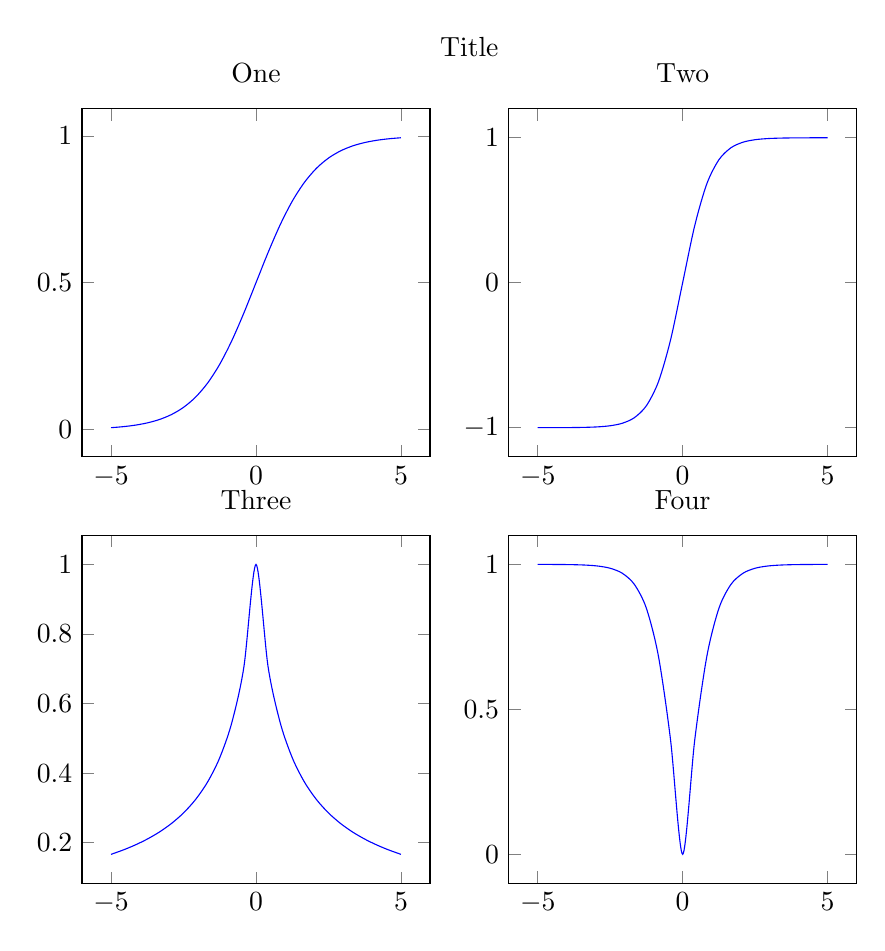
\begin{tikzpicture}
  	\begin{groupplot}[group style={group size=2 by 2},height=6cm,width=6cm]
    		\nextgroupplot[title=One]
    		\addplot[blue,smooth] {1/(1+exp(-x))};
    		\nextgroupplot[title=Two]
    		\addplot[blue,smooth] {tanh(x)};
    		\nextgroupplot[title=Three]
   		\addplot[blue,smooth] {1/(1 + abs(x))};
    		\nextgroupplot[title=Four]
    		\addplot[blue,smooth] {abs(tanh(x))};
  	\end{groupplot}
	\node (title) at ($(group c1r1.center)!0.5!(group c2r1.center)+(0,3cm)$) {Title};
\end{tikzpicture}

\end{document}